\documentclass[12pt,a4paper]{ctexrep}

\usepackage[a4paper,margin=2.6cm]{geometry}
\usepackage{amsmath,amssymb,amsthm,mathtools,bm}
\usepackage{physics}
\usepackage{booktabs}
\usepackage{array}
\usepackage{enumitem}
\usepackage{hyperref}
\usepackage{longtable}
\usepackage{float}
\usepackage{tikz}

\hypersetup{
  colorlinks=true,
  linkcolor=blue,
  urlcolor=blue,
  citecolor=blue
}

\title{日地系统的理论分析与数值模拟}
\author{}
\date{}

\newtheorem*{remark}{说明}
\newtheorem*{example}{例}
\newtheorem*{algorithmidea}{算法思想}

\begin{document}

\maketitle

\begin{abstract}
本文日地系统的轨道方程和数值模拟。从完整牛顿方程出发，导出相对运动方程与质心表示，讨论圆轨道解及固定太阳近似。
在此基础上，继续讨论日地系统的数值模拟。包括从相对运动系出发建立二维与三维数值模型，
 Euler 方法与 Velocity-Verlet 方法的原理、实现和适用性，以及二者在圆轨道上的数值对比实验。
 最后，讨论如何以太阳--地月系质心（Sun--EM Bary）为对象，用 JPL Horizons 数据作为参考y，对数值模拟结果作定量验证。
\end{abstract}

\tableofcontents

\chapter{日地系统的理论分析}

\section{问题背景}

为了研究火箭或探测器在日地系统中的运动，最自然的第一步并不是立刻把推力、变质量和摄动全部放入模型，
而是先把日地系统本身的动力学结构写清楚。若能先把太阳和地球之间的相对运动还原为一个标准二体问题，
那么后续的轨道设计与数值模拟都会更清晰\cite{MurrayDermott1999,BateMuellerWhite1971}。

本章的目标是：
\begin{enumerate}[label=\arabic*.]
  \item 写出太阳和地球在万有引力作用下的完整运动方程；
  \item 将该系统化为一个关于相对位置的中心力二体问题；
  \item 说明质心坐标下太阳与地球的位置表达；
  \item 给出圆轨道的特解及其周期公式；
  \item 说明固定太阳近似的依据。
\end{enumerate}

\section{日地系统的完整牛顿方程}

设
\[
M_S>0,\qquad M_E>0
\]
分别表示太阳和地球的质量，
\[
\bm r_S(t),\qquad \bm r_E(t)\in \mathbb R^3
\]
分别表示时刻 \(t\) 太阳和地球在某惯性参考系中的位置向量。

记万有引力常数为 \(G\)。根据牛顿万有引力定律\cite{MurrayDermott1999,BateMuellerWhite1971}，
太阳受到地球的引力为
\[
\bm F_{S\leftarrow E}
=
G M_S M_E
\frac{\bm r_E-\bm r_S}{\|\bm r_E-\bm r_S\|^3},
\]
地球受到太阳的引力为
\[
\bm F_{E\leftarrow S}
=
G M_S M_E
\frac{\bm r_S-\bm r_E}{\|\bm r_E-\bm r_S\|^3}.
\]
由牛顿第二定律得
\begin{equation}\label{eq:sun-motion}
M_S \ddot{\bm r}_S
=
G M_S M_E
\frac{\bm r_E-\bm r_S}{\|\bm r_E-\bm r_S\|^3},
\end{equation}
\begin{equation}\label{eq:earth-motion}
M_E \ddot{\bm r}_E
=
G M_S M_E
\frac{\bm r_S-\bm r_E}{\|\bm r_E-\bm r_S\|^3}.
\end{equation}

将质量约去，可写为
\begin{equation}\label{eq:sun-motion-2}
\ddot{\bm r}_S
=
G M_E
\frac{\bm r_E-\bm r_S}{\|\bm r_E-\bm r_S\|^3},
\end{equation}
\begin{equation}\label{eq:earth-motion-2}
\ddot{\bm r}_E
=
G M_S
\frac{\bm r_S-\bm r_E}{\|\bm r_E-\bm r_S\|^3}.
\end{equation}

这是一个耦合的二阶非线性常微分方程组，描述太阳和地球在相互引力作用下的运动。

\section{相对运动方程的导出}

由于在双体系统中真正重要的是两个天体之间的相对位置，因此引入
\[
\bm r(t)=\bm r_E(t)-\bm r_S(t).
\]
于是
\[
\ddot{\bm r}(t)=\ddot{\bm r}_E(t)-\ddot{\bm r}_S(t).
\]
将 \eqref{eq:sun-motion-2} 和 \eqref{eq:earth-motion-2} 代入，得到
\begin{align*}
\ddot{\bm r}
&=
G M_S \frac{\bm r_S-\bm r_E}{\|\bm r_E-\bm r_S\|^3}
-
G M_E \frac{\bm r_E-\bm r_S}{\|\bm r_E-\bm r_S\|^3}.
\end{align*}
注意到
\[
\bm r_S-\bm r_E=-(\bm r_E-\bm r_S)=-\bm r,
\qquad
\bm r_E-\bm r_S=\bm r,
\]
故
\begin{align*}
\ddot{\bm r}
&=
- G M_S \frac{\bm r}{\|\bm r\|^3}
- G M_E \frac{\bm r}{\|\bm r\|^3} \\
&=
- G(M_S+M_E)\frac{\bm r}{\|\bm r\|^3}.
\end{align*}
因此相对运动满足
\begin{equation}\label{eq:relative-motion}
\ddot{\bm r}
=
- G(M_S+M_E)\frac{\bm r}{\|\bm r\|^3}.
\end{equation}
若记
\[
\mu:=G(M_S+M_E),
\]
则可简写为
\begin{equation}\label{eq:relative-motion-mu}
\ddot{\bm r}=-\mu \frac{\bm r}{\|\bm r\|^3}.
\end{equation}

这一步把原来的耦合双体系统化为了一个标准的中心力二体问题\cite{MurrayDermott1999,BateMuellerWhite1971}。
以后无论是理论分析还是数值模拟，都可以直接围绕 \eqref{eq:relative-motion-mu} 展开。

\section{质心运动与质心坐标表达}

定义日地系统的质心为
\[
\bm R_c(t)=\frac{M_S\bm r_S(t)+M_E\bm r_E(t)}{M_S+M_E}.
\]
对其求二阶导数，得
\[
(M_S+M_E)\ddot{\bm R}_c=M_S\ddot{\bm r}_S+M_E\ddot{\bm r}_E.
\]
若将日-地系统视为孤立系统，由 \eqref{eq:sun-motion} 和 \eqref{eq:earth-motion} 可知右边恰好为零，因此
\[
\ddot{\bm R}_c=0.
\]
所以质心作匀速直线运动；特别地，若选取质心静止系，则可取\cite{MurrayDermott1999,BateMuellerWhite1971}
\[
\bm R_c=0.
\]

在质心系中，由
\[
M_S \bm r_S + M_E \bm r_E = 0,
\qquad
\bm r = \bm r_E-\bm r_S
\]
可解得
\begin{equation}\label{eq:rs-bary}
\bm r_S=-\frac{M_E}{M_S+M_E}\bm r,
\end{equation}
\begin{equation}\label{eq:re-bary}
\bm r_E=\frac{M_S}{M_S+M_E}\bm r.
\end{equation}

取模可得
\[
r_S=\frac{M_E}{M_S+M_E}\,r,
\qquad
r_E=\frac{M_S}{M_S+M_E}\,r,
\]
其中 \(r=\|\bm r\|\) 表示日地之间的相对距离。因此
\[
\frac{r_S}{r_E}=\frac{M_E}{M_S}.
\]

在实际天体力学计算中，往往直接使用标准引力参数 \(GM\) 而不是单独使用质量 \(M\)\cite{JPLAstroParameters}，因为运动方程本身直接依赖于 \(GM\)，而且观测上 \(GM\) 的精度通常更高。于是
\[
\frac{M_E}{M_S}=\frac{GM_E}{GM_S}.
\]
若取太阳和地球的标准引力参数，便可估计质心离太阳中心极近，太阳只作极小幅度摆动，而地球几乎绕着该质心作完整的天文单位尺度运动。

\section{圆轨道作为特殊解}

下面考虑 \eqref{eq:relative-motion-mu} 的一个特殊解：圆轨道。

设日地相对距离恒为常数 \(a>0\)，且轨道位于某一固定平面内。取该平面为 \(xy\)-平面，设
\begin{equation}\label{eq:circular-ansatz}
\bm r(t)
=
a
\begin{pmatrix}
\cos nt\\
\sin nt\\
0
\end{pmatrix},
\end{equation}
其中 \(n>0\) 为常数角速度。则
\[
\ddot{\bm r}(t)=-n^2\bm r(t).
\]
另一方面，由于 \(\|\bm r(t)\|=a\)，方程 \eqref{eq:relative-motion-mu} 右端为
\[
-\mu \frac{\bm r(t)}{\|\bm r(t)\|^3}=-\mu \frac{\bm r(t)}{a^3}.
\]
因此必须有
\[
-n^2\bm r(t)=-\mu \frac{\bm r(t)}{a^3},
\]
从而得到
\begin{equation}\label{eq:n2}
n^2=\frac{\mu}{a^3}=\frac{G(M_S+M_E)}{a^3}.
\end{equation}
于是圆轨道周期为
\begin{equation}\label{eq:period}
T=\frac{2\pi}{n}=2\pi \sqrt{\frac{a^3}{G(M_S+M_E)}}.
\end{equation}
这正是二体问题中的 Kepler 第三定律形式\cite{MurrayDermott1999,BateMuellerWhite1971}。

\section{固定太阳近似的来源}

在日地系统中，太阳质量远大于地球质量，查找相关数据，太阳和地球的标准引力参数分别为\cite{JPLAstroParameters}
\[
GM_S=1.32712440041279419\times 10^{11}\ \mathrm{km^3\,s^{-2}},
\qquad
GM_E=398600.435507\ \mathrm{km^3\,s^{-2}},
\]
得
\[
\frac{r_S}{r_E}
=
\frac{M_E}{M_S}
=
\frac{GM_E}{GM_S}
\approx 3.00349\times 10^{-6}.
\]
也就是说，
\[
r_S \approx 3.0\times 10^{-6}\, r_E,
\]
太阳绕质心的运动尺度只有地球的约三百万分之一。

因此
\[
M_S\gg M_E,
\qquad
M_S+M_E\approx M_S.
\]
于是相对运动方程 \eqref{eq:relative-motion-mu} 近似为
\begin{equation}\label{eq:approx-relative}
\ddot{\bm r}\approx -GM_S\frac{\bm r}{\|\bm r\|^3}.
\end{equation}
如果再进一步把太阳近似固定在原点，即令
\[
\bm r_S(t)\approx 0,
\qquad
\bm r_E(t)\approx \bm r(t),
\]
则地球运动可近似写成
\begin{equation}\label{eq:earth-around-fixed-sun}
\ddot{\bm r}_E=-GM_S\frac{\bm r_E}{\|\bm r_E\|^3}.
\end{equation}

这就是通常所谓的“地球绕固定太阳运动”模型\cite{MurrayDermott1999,BateMuellerWhite1971}。
它不是最原始的精确模型，而是从完整日地二体系统经过 \(M_S\gg M_E\) 
这一物理近似后得到的。

\section{本章小结}

综上，日地系统的理论结构可以概括为：
\begin{enumerate}[label=\arabic*.]
  \item 在惯性系中，太阳和地球满足耦合的牛顿方程；
  \item 引入相对位置 \(\bm r=\bm r_E-\bm r_S\) 后，系统化为中心力二体方程 \eqref{eq:relative-motion-mu}；
  \item 在质心系中，太阳和地球的位置由 \eqref{eq:rs-bary}--\eqref{eq:re-bary} 给出；
  \item 圆轨道是该系统的显式特解，其角速度和周期满足 \eqref{eq:n2}--\eqref{eq:period}；
  \item 固定太阳模型是 \(M_S\gg M_E\) 下的近似模型。
\end{enumerate}

因此，第二章的数值模拟将以相对运动方程为基础展开。

\chapter{日地系统的数值模拟}

\section{从相对运动系开始的数值模拟框架}

由第一章可知，日地系统在质心系中的内部动力学由
\[
\ddot{\bm r}=-\mu \frac{\bm r}{\|\bm r\|^3},
\qquad
\mu=G(M_S+M_E)
\]
决定，其中 \(\bm r=\bm r_E-\bm r_S\) 表示地球相对太阳的位置向量。
数值模拟时，不必直接积分 \(\bm r_S,\bm r_E\) 两组耦合方程，而是先积分 \(\bm r\)，再由
\[
\bm r_S=-\frac{M_E}{M_S+M_E}\bm r,
\qquad
\bm r_E=\frac{M_S}{M_S+M_E}\bm r
\]
恢复太阳和地球在质心系中的位置\cite{MurrayDermott1999,BateMuellerWhite1971}。

这种做法的优点是：
\begin{enumerate}[label=\arabic*.]
  \item 消除了不必要的整体平移自由度；
  \item 直接抓住了引力作用依赖的相对位置；
  \item 更便于讨论能量、角动量与轨道几何；
  \item 便于将二维模型推广到三维模型。
\end{enumerate}

\section{二维模型与无量纲化}

若先在固定平面内模拟，例如取 \(xy\)-平面，则令
\[
\bm r(t)=(x(t),y(t)).
\]
方程化为\cite{BateMuellerWhite1971}
\begin{equation}\label{eq:2d-second}
\ddot x=-\mu \frac{x}{(x^2+y^2)^{3/2}},
\qquad
\ddot y=-\mu \frac{y}{(x^2+y^2)^{3/2}}.
\end{equation}

令
\[
v_x=\dot x,\qquad v_y=\dot y,
\]
则可写成一阶系统
\begin{equation}\label{eq:2d-first}
\dot x=v_x,\qquad \dot y=v_y,
\end{equation}
\begin{equation}\label{eq:2d-first-2}
\dot v_x=-\mu \frac{x}{(x^2+y^2)^{3/2}},
\qquad
\dot v_y=-\mu \frac{y}{(x^2+y^2)^{3/2}}.
\end{equation}

为简化数值实验，下面先使用无量纲单位：
\begin{itemize}
  \item 长度单位取 \(1\,\mathrm{AU}\)；
  \item 时间单位取 \(1\,\mathrm{year}\)；
  \item 令地球平均轨道半径近似为 \(1\)；
  \item 令地球绕太阳一周的周期近似为 \(1\)。
\end{itemize}
在此单位制下，圆轨道条件给出
\[
\mu=4\pi^2.
\]
这时圆轨道的一个标准初值为
\begin{equation}\label{eq:circular-ic}
x(0)=1,\qquad y(0)=0,\qquad v_x(0)=0,\qquad v_y(0)=2\pi.
\end{equation}
理论解为
\[
x(t)=\cos(2\pi t),\qquad y(t)=\sin(2\pi t).
\]

\begin{figure}[htbp]
\centering
\begin{tikzpicture}[scale=3]

  % 坐标轴
  \draw[->, thin] (-1.3,0) -- (1.35,0) node[below right] {$x$};
  \draw[->, thin] (0,-1.3) -- (0,1.35) node[left] {$y$};

  % 单位圆轨道
  \draw[thick, blue] (0,0) circle (1);

  % 太阳
  \filldraw[orange] (0,0) circle (0.035);
  \node[below right] at (0,0) [orange]{太阳};

  % 初始点
  \filldraw[blue] (1,0) circle (0.03);
  \node[below right] at (1,0) {$\bigl(1,0\bigr)$};

  % 初速度箭头
  \draw[->, very thick, blue] (1,0) -- (1,0.45);
  \node[right] at (1,0.48) [blue]{$\bm v(0)=(0,2\pi)$};

  % 轨道方向箭头
  \draw[->, thick, blue] (0.55,0.84) arc[start angle=57,end angle=77,radius=1];

  % 单位圆标注
  \node[blue] at (-0.7,1.00) {$x^2+y^2=1$};

  % 原点标注
  \node[below left] at (0,0) {$O$};

  % 地球标注
  \node[above right] at (1,0) [blue]{地球};


\end{tikzpicture}
\caption{二维无量纲模型下的圆轨道初值示意图。地球初始位置取为 \((1,0)\)，初始速度竖直向上，
故轨道为逆时针方向的单位圆。}
\label{fig:circular-ic}
\end{figure}

由初值
\[
x(0)=1,\qquad y(0)=0,\qquad v_x(0)=0,\qquad v_y(0)=2\pi,
\]
可知轨道从点 \((1,0)\) 出发，并沿逆时针方向绕单位圆运动，这与理论解
\[
x(t)=\cos(2\pi t),\qquad y(t)=\sin(2\pi t)
\]
完全一致。

\section{Euler 方法的原理与应用}

\subsection{Euler 方法的基本思想}

Euler 方法来源于最简单的一阶 Taylor 截断\cite{HairerLubichWanner2006,LeimkuhlerReich2004}。对一阶系统
\[
\dot Y=f(Y)
\]
在时刻 \(t_n\) 处作展开，得到
\[
Y(t_{n+1})=Y(t_n)+h f(Y(t_n))+O(h^2),
\]
其中 \(h=t_{n+1}-t_n\) 为时间步长。因此，舍去高阶项后得到显式 Euler 格式
\begin{equation}\label{eq:euler-general}
Y_{n+1}=Y_n+h f(Y_n).
\end{equation}

将 \eqref{eq:2d-first}--\eqref{eq:2d-first-2} 视为一阶系统，状态向量取为
\[
Y=(x,y,v_x,v_y)^\top,
\]
则 Euler 方法的迭代公式为
\begin{align}
 x_{n+1} &= x_n+h v_{x,n},\label{eq:euler-x}\\
 y_{n+1} &= y_n+h v_{y,n},\label{eq:euler-y}\\
 v_{x,n+1} &= v_{x,n}-h\mu \frac{x_n}{(x_n^2+y_n^2)^{3/2}},\label{eq:euler-vx}\\
 v_{y,n+1} &= v_{y,n}-h\mu \frac{y_n}{(x_n^2+y_n^2)^{3/2}}.\label{eq:euler-vy}
\end{align}

\subsection{Euler 方法在轨道问题中的特点}

Euler 方法的优点是公式极其简单，适合入门、调试和作为对照实验；但在轨道问题中，它有明显缺点：
\begin{enumerate}[label=\arabic*.]
  \item 它只有一阶精度，步长稍大时误差积累很快；
  \item 它不保持哈密顿系统的几何结构（圆形轨道在长期积分中会逐渐变形）；
  \item 在长期传播中，能量往往出现明显漂移（能量不守恒）；
  \item 对周期轨道，常见现象是轨道逐渐向外发散或向内坍缩。
\end{enumerate}
因此，Euler 方法更适合用来说明“一个不适合轨道长期传播的方法会出现什么问题”，而不适合作为正式的轨道长期模拟方法。

\section{Velocity-Verlet 方法的原理与应用}

\subsection{从二阶系统出发}

对于形如
\[
\ddot{\bm r}=\bm a(\bm r)
\]
的二阶系统，其中加速度仅依赖于位置，Velocity-Verlet 是最自然的时间离散格式之一。对于日地相对运动，有
\[
\bm a(\bm r)=-\mu \frac{\bm r}{\|\bm r\|^3}.
\]

\subsection{从 Taylor 展开导出位置更新}

对位置作 Taylor 展开：
\[
\bm r(t+h)=\bm r(t)+h\bm v(t)+\frac{h^2}{2}\bm a(t)+O(h^3).
\]
因此可用
\begin{equation}\label{eq:vv-r}
\bm r_{n+1}=\bm r_n+h\bm v_n+\frac{h^2}{2}\bm a_n
\end{equation}
更新位置，其中 \(\bm a_n=\bm a(\bm r_n)\)。

在得到 \(\bm r_{n+1}\) 后，计算新位置对应的加速度
\[
\bm a_{n+1}=\bm a(\bm r_{n+1}).
\]
然后利用当前与下一步加速度的平均值更新速度：
\begin{equation}\label{eq:vv-v}
\bm v_{n+1}=\bm v_n+\frac{h}{2}(\bm a_n+\bm a_{n+1}).
\end{equation}
这就是 Velocity-Verlet 的基本格式。

\subsection{哈密顿观点下的解释}

对于可分离哈密顿系统
\[
H(q,p)=T(p)+V(q),
\]
Velocity-Verlet 也可视为一种 ``kick--drift--kick'' 的对称分裂：
\[
p^{n+\frac12}=p^n-\frac{h}{2}\nabla V(q^n),
\]
\[
q^{n+1}=q^n+h\,p^{n+\frac12},
\]
\[
p^{n+1}=p^{n+\frac12}-\frac{h}{2}\nabla V(q^{n+1}).
\]
因此，对固定步长的可分离保守系统，Velocity-Verlet 是一个二阶、时间可逆、保辛的积分格式。它一般并不在每一步严格守恒原始能量，但常见现象是：长期积分中能量误差呈有界振荡，而不是像 Euler 方法那样持续漂移。

\subsection{二维情形下的具体实现}

对二维状态 \(\bm r_n=(x_n,y_n)\)、\(\bm v_n=(v_{x,n},v_{y,n})\)，加速度函数为
\[
\bm a(\bm r)=
-\mu \frac{\bm r}{\|\bm r\|^3}
=
\left(
-\mu \frac{x}{(x^2+y^2)^{3/2}},
-\mu \frac{y}{(x^2+y^2)^{3/2}}
\right).
\]
因此每一步迭代为
\[
\bm a_n=\bm a(\bm r_n),
\]
\[
\bm r_{n+1}=\bm r_n+h\bm v_n+\frac{h^2}{2}\bm a_n,
\]
\[
\bm a_{n+1}=\bm a(\bm r_{n+1}),
\]
\[
\bm v_{n+1}=\bm v_n+\frac{h}{2}(\bm a_n+\bm a_{n+1}).
\]

\section{圆轨道上 Euler 与 Velocity-Verlet 的对比实验}

\subsection{实验设置}

为了直接比较两种方法，考虑圆轨道初值 \eqref{eq:circular-ic}，模拟一整年（即一个完整周期），比较：
\begin{enumerate}[label=\arabic*.]
  \item 一周后终点与理论点 \((1,0)\) 的位置误差；
  \item 相对能量误差 \( |E_N-E_0|/|E_0| \)；
  \item 相对角动量误差 \( |L_N-L_0|/|L_0| \)。
\end{enumerate}
其中
\[
E=\frac12(v_x^2+v_y^2)-\frac{\mu}{\sqrt{x^2+y^2}},
\qquad
L=xv_y-yv_x.
\]

\subsection{一个具体数值例子}

取两组典型步长 \(h=10^{-2}\) 与 \(h=10^{-3}\)，数值实验结果可整理为表 \ref{tab:euler-vv-circle}。

\begin{table}[H]
\centering
\caption{圆轨道上一周期后 Euler 与 Velocity-Verlet 的对比}
\label{tab:euler-vv-circle}
\begin{tabular}{cccccc}
\toprule
方法 & 步长 \(h\) & 位置误差 & 相对能量误差 & 相对角动量误差 & 现象 \\
\midrule
Euler & $10^{-2}$ & $2.2556$ & $3.4845\times 10^{-1}$ & $2.2650\times 10^{-1}$ & 轨道明显发散 \\
Velocity-Verlet & $10^{-2}$ & $8.2560\times 10^{-3}$ & $4.2229\times 10^{-12}$ & $1.4136\times 10^{-16}$ & 仍接近圆轨道 \\
Euler & $10^{-3}$ & $3.5853\times 10^{-1}$ & $6.8360\times 10^{-2}$ & $3.6033\times 10^{-2}$ & 漂移仍明显 \\
Velocity-Verlet & $10^{-3}$ & $8.2682\times 10^{-5}$ & $5.3995\times 10^{-15}$ & $2.6858\times 10^{-15}$ & 结果极稳定 \\
\bottomrule
\end{tabular}
\end{table}

\begin{figure}[H]
\centering
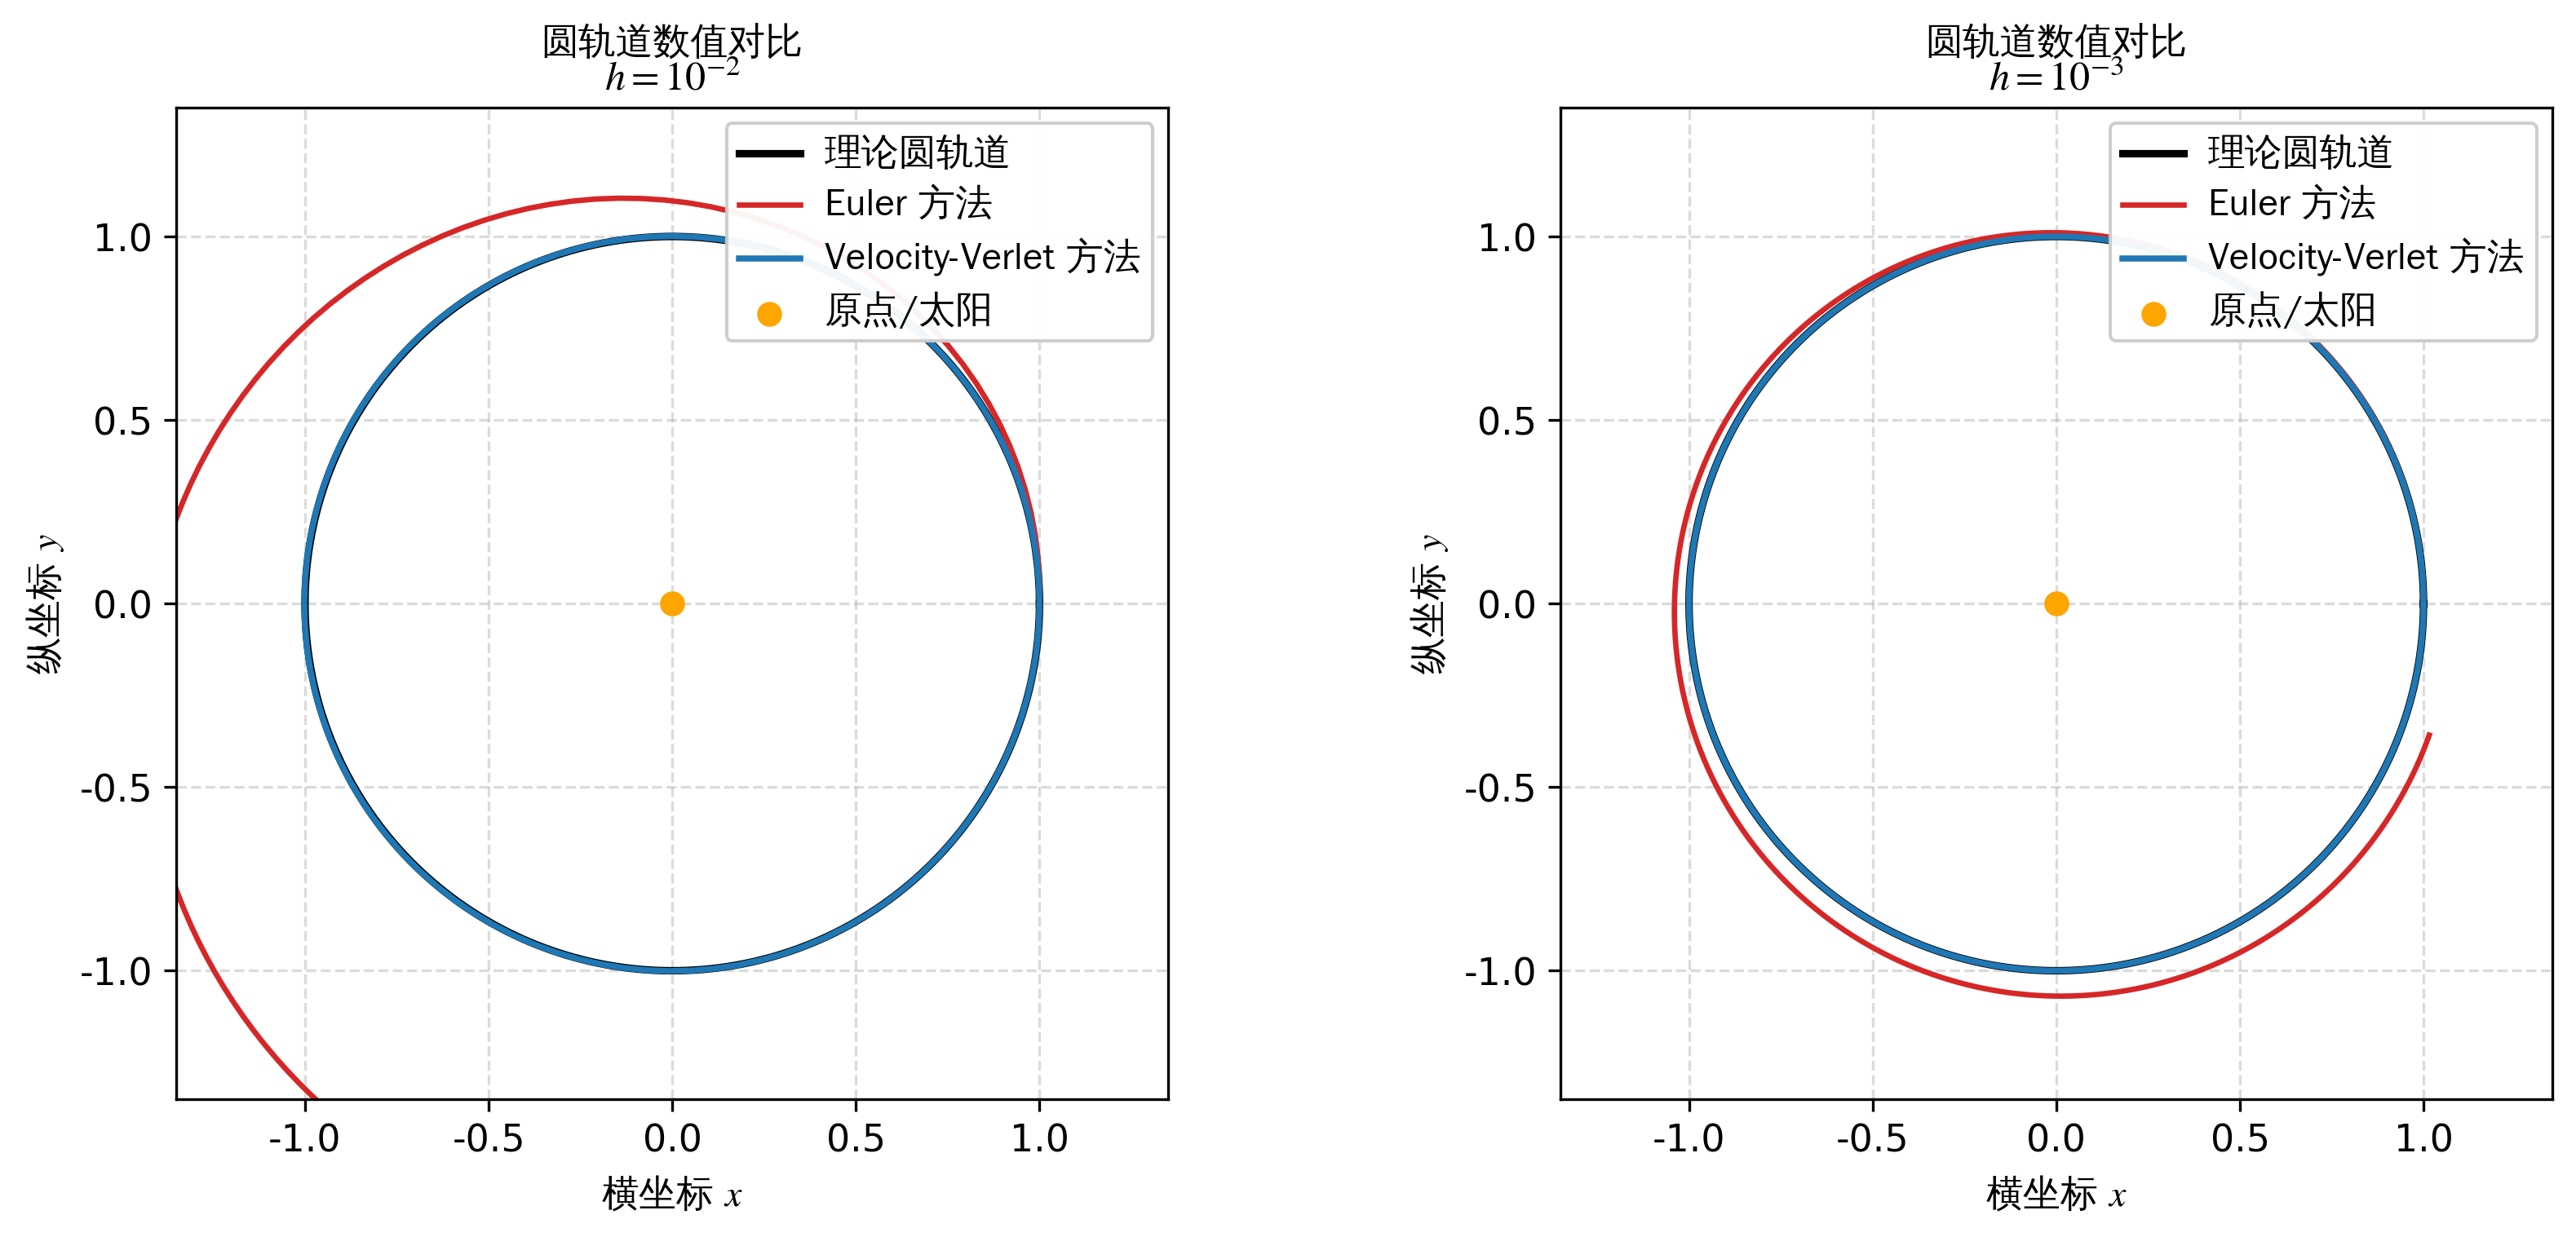
\includegraphics[width=0.92\textwidth]{images/circle_orbit_comparison.png}
\caption{圆轨道上一周期内的数值轨道对比。左图对应步长 \(h=10^{-2}\)，右图对应步长 \(h=10^{-3}\)。黑色曲线为理论圆轨道，红色曲线为 Euler 方法得到的数值轨道，蓝色曲线为 Velocity-Verlet 方法得到的数值轨道，橙色点表示原点处的太阳。可以看到，当步长较大时，Euler 方法出现明显轨道漂移，而 Velocity-Verlet 方法仍能较好保持圆轨道结构；当步长减小到 \(10^{-3}\) 时，两者误差均减小，但 Velocity-Verlet 方法仍明显更稳定。}
\label{fig:circle-orbit-comparison}
\end{figure}

\begin{figure}[H]
\centering
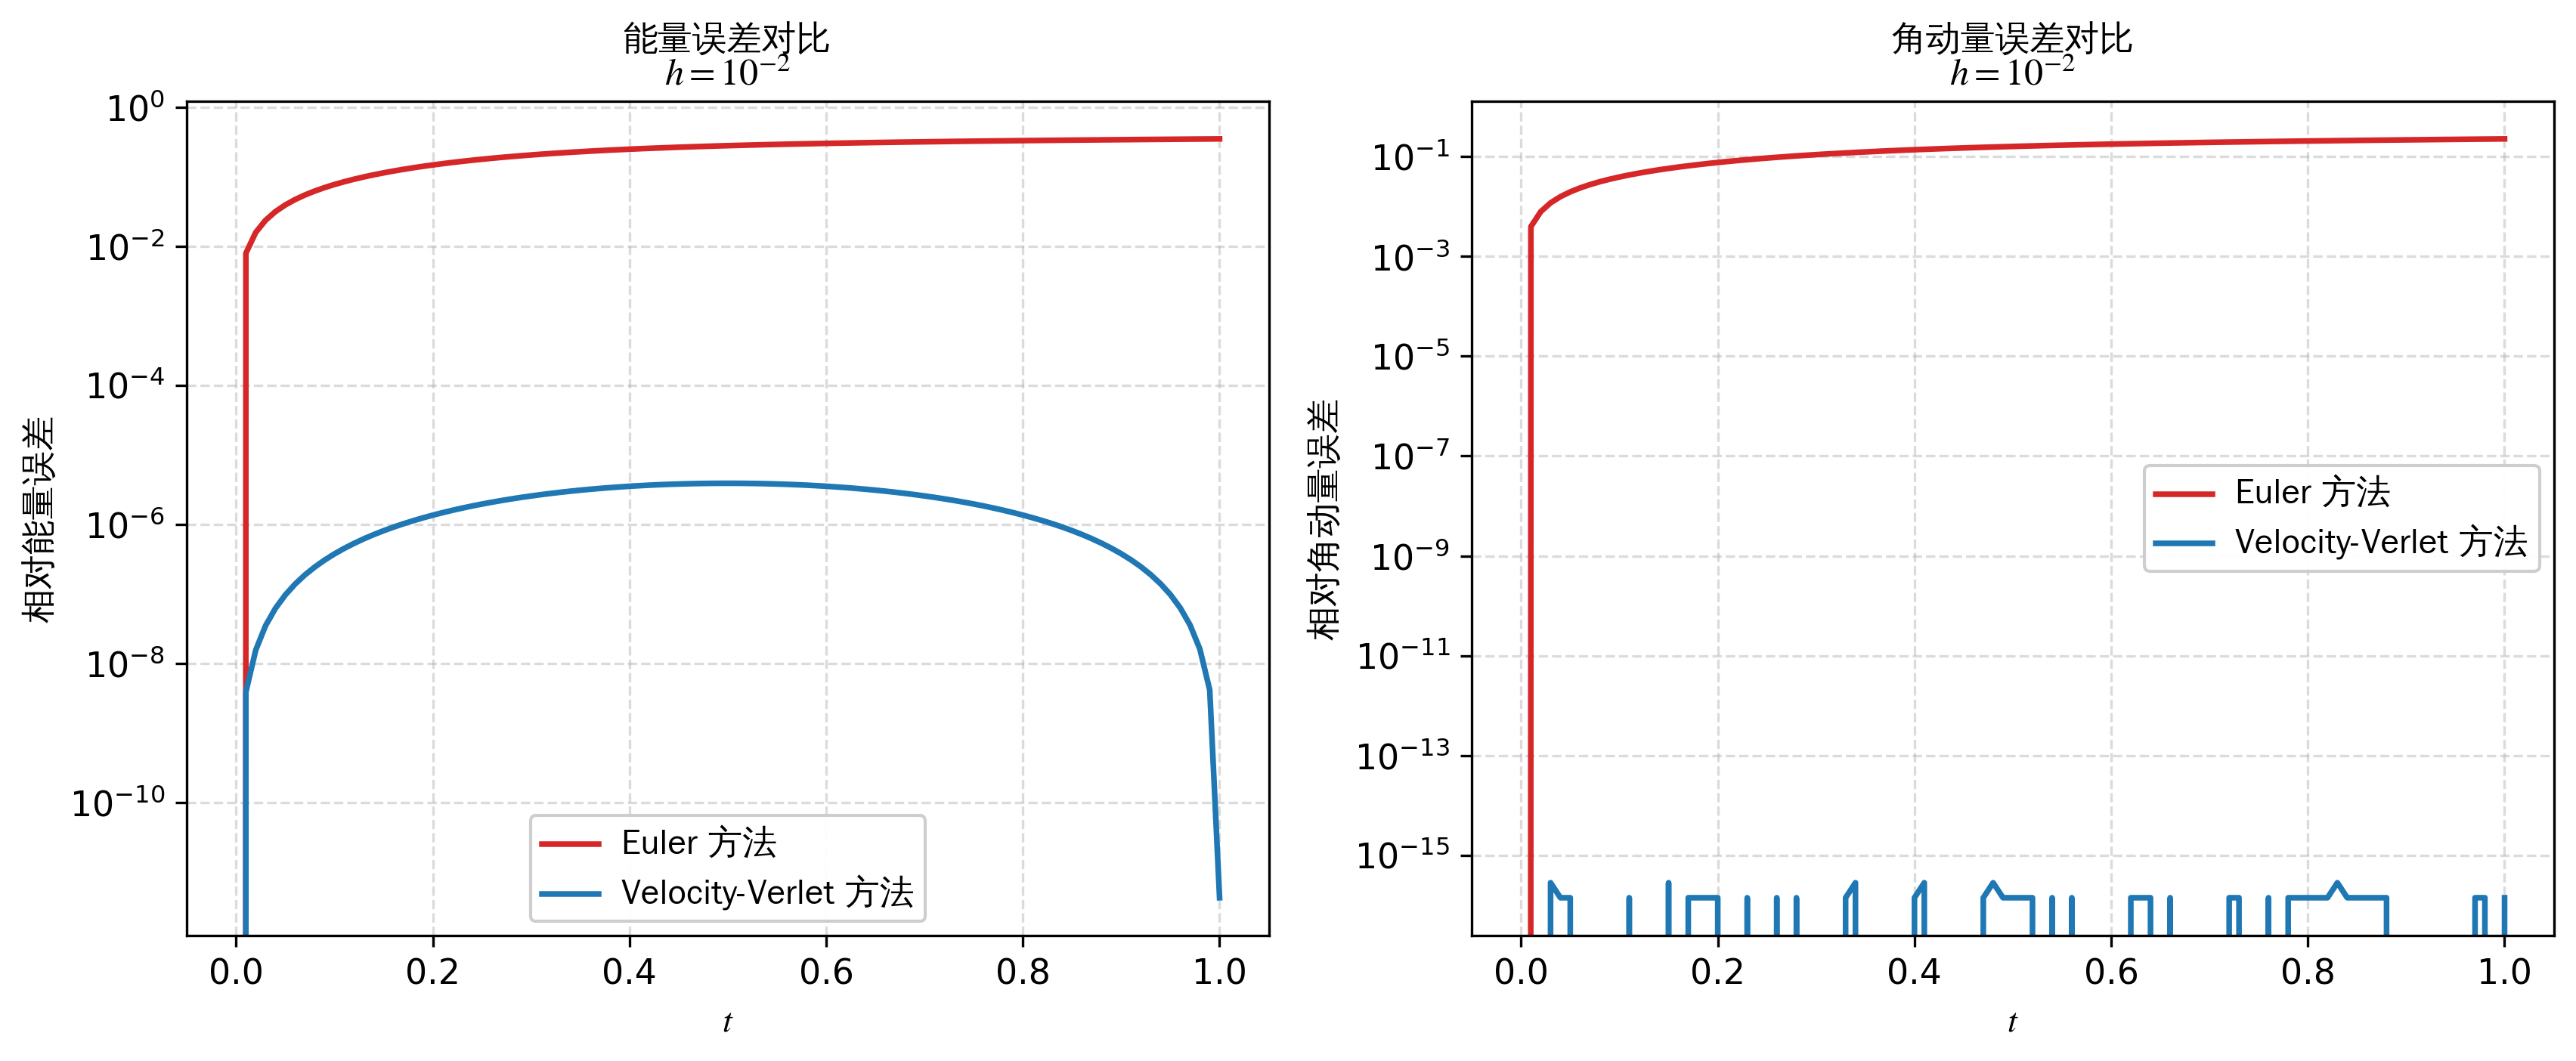
\includegraphics[width=0.92\textwidth]{images/conservation_errors_h1e-02.png}
\caption{步长 \(h=10^{-2}\) 时的守恒量误差对比。左图为相对能量误差，右图为相对角动量误差。红色曲线对应 Euler 方法，蓝色曲线对应 Velocity-Verlet 方法。可以看到，Euler 方法的能量误差和角动量误差都随时间迅速累积，而 Velocity-Verlet 方法在同样步长下仍能将误差控制在极小范围内，说明其在保守轨道问题中具有更好的长期稳定性。}
\label{fig:conservation-errors-h1e-2}
\end{figure}

\begin{figure}[H]
\centering
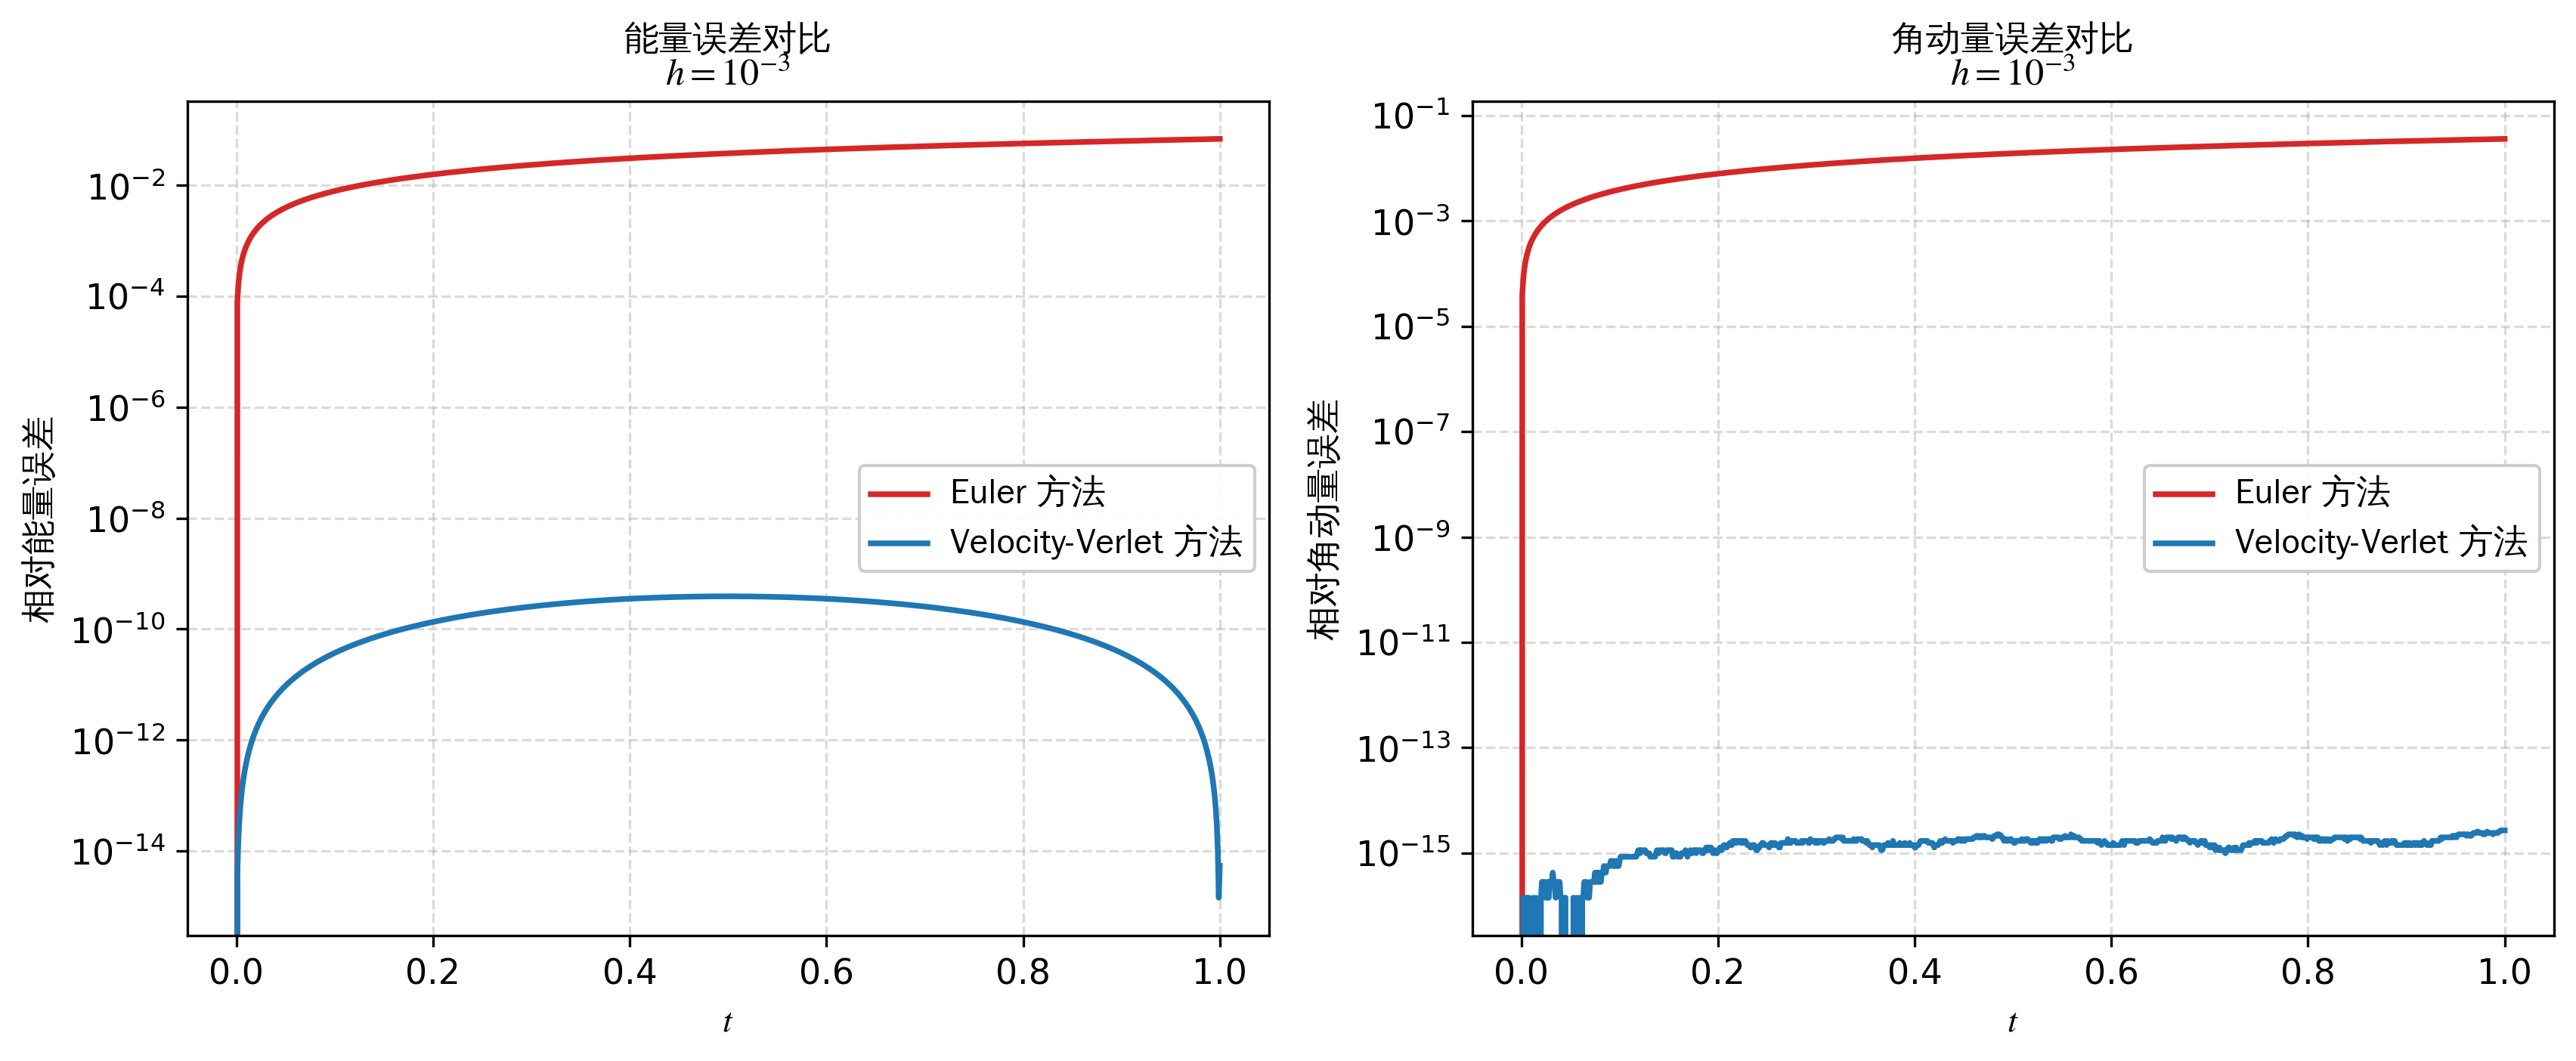
\includegraphics[width=0.92\textwidth]{images/conservation_errors_h1e-03.png}
\caption{步长 \(h=10^{-3}\) 时的守恒量误差对比。左图为相对能量误差，右图为相对角动量误差。与 \(h=10^{-2}\) 的情形相比，减小步长后两种方法的误差都进一步降低；但仍可明显看出，Euler 方法存在较显著的误差积累，而 Velocity-Verlet 方法的误差始终维持在接近机器精度的水平，反映出其在圆轨道长期传播中的优越表现。}
\label{fig:conservation-errors-h1e-3}
\end{figure}

从图 \ref{fig:circle-orbit-comparison} 可以直观看出，在圆轨道初值下，两种数值方法的表现存在明显差异。当步长取为 \(h=10^{-2}\) 时，Euler 方法得到的轨道已经明显偏离理论圆轨道，出现了较强的外扩漂移；相比之下，Velocity-Verlet 方法得到的轨道仍与理论圆轨道几乎重合，说明其在相同步长下具有更好的几何稳定性。当步长减小到 \(h=10^{-3}\) 时，Euler 方法的轨道误差虽然有所减小，但仍能观察到明显偏离；而 Velocity-Verlet 方法则继续保持了与理论圆轨道高度一致的数值结果。

这种差异在守恒量误差图中表现得更加清楚。由图 \ref{fig:conservation-errors-h1e-2} 可见，在较大步长 \(h=10^{-2}\) 下，Euler 方法的相对能量误差和相对角动量误差都随时间迅速增长，说明该方法在长期传播中会持续破坏系统的守恒结构；而 Velocity-Verlet 方法的误差始终维持在极小量级，表现出显著更好的稳定性。进一步地，从图 \ref{fig:conservation-errors-h1e-3} 可以看到，当步长减小到 \(h=10^{-3}\) 时，两种方法的误差都降低了，但 Euler 方法仍然存在明显的误差累积趋势，而 Velocity-Verlet 方法的能量误差与角动量误差依旧保持在接近机器精度的范围内。

综合这三张图可以得出结论：对于本文所研究的圆轨道保守系统，Euler 方法虽然实现最为简单，但数值耗散（或增益）效应较明显，难以在较长时间传播中保持轨道结构与守恒量；Velocity-Verlet 方法则能够在较低计算复杂度下更好地保持轨道几何形状，并有效控制能量与角动量误差，因此更适合作为本文后续日地系统数值模拟的基础方法。


\section{三维模型的推广}

\subsection{三维相对运动方程}

在三维情形下\cite{MurrayDermott1999,BateMuellerWhite1971}，取
\[
\bm r(t)=(x(t),y(t),z(t)),
\qquad
\bm v(t)=(v_x(t),v_y(t),v_z(t)).
\]
则相对运动方程为
\[
\ddot{\bm r}=-\mu \frac{\bm r}{\|\bm r\|^3},
\qquad
\|\bm r\|=\sqrt{x^2+y^2+z^2}.
\]
对应的一阶系统为
\[
\dot x=v_x,\quad \dot y=v_y,\quad \dot z=v_z,
\]
\[
\dot v_x=-\mu \frac{x}{(x^2+y^2+z^2)^{3/2}},\qquad
\dot v_y=-\mu \frac{y}{(x^2+y^2+z^2)^{3/2}},\qquad
\dot v_z=-\mu \frac{z}{(x^2+y^2+z^2)^{3/2}}.
\]

\subsection{三维模拟的意义}

从理论上说，二体问题总是限制在某个平面内，因此三维模型并不比二维更“本质复杂”；
但三维模拟仍然很有意义，因为它能够：
\begin{enumerate}[label=\arabic*.]
  \item 显式处理轨道倾角；
  \item 便于与 JPL 提供的三维状态向量直接对接\cite{JPLHorizonsManual}；
  \item 为以后加入摄动、多体效应和坐标变换做准备。
\end{enumerate}

例如，可取
\[
\bm r(0)=(1,0,0),
\qquad
\bm v(0)=\left(0,2\pi\cos i,2\pi\sin i\right),
\]
其中 \(i\) 为给定倾角。这样得到的轨道不再落在 \(xy\)-平面中，而是位于一个倾斜的轨道平面内。

\subsection{三维下的守恒量}

三维情形下的机械能仍为\cite{MurrayDermott1999}
\[
E=\frac12\|\bm v\|^2-\frac{\mu}{\|\bm r\|},
\]
角动量变为向量
\[
\bm L=\bm r\times \bm v.
\]
因此数值模拟时，除观察 \(E\) 是否近似守恒外，还应检查 \(\bm L\) 的模长及其方向是否近似不变。

\subsection{三维下的 Velocity-Verlet}

Velocity-Verlet 在三维中的形式与二维完全平行：
\[
\bm a(\bm r)=-\mu \frac{\bm r}{\|\bm r\|^3},
\]
\[
\bm a_n=\bm a(\bm r_n),
\]
\[
\bm r_{n+1}=\bm r_n+h\bm v_n+\frac{h^2}{2}\bm a_n,
\]
\[
\bm a_{n+1}=\bm a(\bm r_{n+1}),
\]
\[
\bm v_{n+1}=\bm v_n+\frac{h}{2}(\bm a_n+\bm a_{n+1}).
\]
因此程序结构几乎无需改变，只需把二维向量升级为三维向量即可\cite{HairerLubichWanner2006,LeimkuhlerReich2004}。

\section{实际太阳--地月系质心系统的模拟与 JPL 数据对比}

\subsection{为何选择 Sun--EM Bary 作为比较对象}

为了把简单的二体模型和真实天体数据联系起来，最自然的比较对象不是“太阳--地球中心”，而是“太阳--地月系质心（Sun--EM Bary）”。原因是：真实的地球会受到月球影响而围绕地月系质心摆动，而 JPL 在行星近似位置表和 Horizons 系统中都把 Earth--Moon Barycenter 作为标准对象之一。这样做既更接近真实太阳系动力学，也更便于调用官方星历数据。

为避免记号混淆，本节将“实际系统”理解为太阳与地月系质心之间的相对运动\cite{JPLHorizonsManual,JPLApproximatePositions}。其引力参数取为
\[
\mu_{\mathrm{SEMB}}=GM_{\odot}+GM_{\oplus}+GM_{\mathrm{Moon}}.
\]

\subsection{与 JPL Horizons 对接的基本思路}

JPL Horizons 可以输出某一天体相对于另一参考中心的笛卡尔状态向量或振荡轨道要素。
对于 Sun--EM Bary 系统，可令目标体为 Earth--Moon Barycenter，参考中心为 Sun，
然后获取某个历元的状态向量\cite{JPLHorizonsManual,JPLHorizonsAPI}
\[
\bm r_0=(x_0,y_0,z_0),
\qquad
\bm v_0=(v_{x,0},v_{y,0},v_{z,0}).
\]
然后：
\begin{enumerate}[label=\arabic*.]
  \item 在三维二体模型中，以 \((\bm r_0,\bm v_0)\) 作为初值进行积分；
  \item 若要得到二维模型，则把该状态向量投影到选定参考平面（通常取黄道平面）；
  \item 在后续时刻 \(t_n\) 上，把数值解 \((\bm r_n,\bm v_n)\) 与 Horizons 给出的参考状态作比较。
\end{enumerate}

设计实验比较以下几个量：

\begin{enumerate}[label=\arabic*.]
  \item 位置误差
  \[
  \varepsilon_r(t_n)=\|\bm r_{\mathrm{num}}(t_n)-\bm r_{\mathrm{JPL}}(t_n)\|;
  \]
  \item 速度误差
  \[
  \varepsilon_v(t_n)=\|\bm v_{\mathrm{num}}(t_n)-\bm v_{\mathrm{JPL}}(t_n)\|;
  \]
  \item 若只比较二维投影，还可比较平面角位置误差
  \[
  \varepsilon_\lambda(t_n)=|\lambda_{\mathrm{num}}(t_n)-\lambda_{\mathrm{JPL}}(t_n)|;
  \]
  \item 对于径向变化明显的情形，还可比较日距误差
  \[
  \varepsilon_\rho(t_n)=\left|\,\|\bm r_{\mathrm{num}}(t_n)\|-\|\bm r_{\mathrm{JPL}}(t_n)\|\right|.
  \]
\end{enumerate}

需要指出的是：二维相对运动模型本质上是一个固定平面内的二体模型，而 JPL Horizons 背后使用的是高精度太阳系星历。因此，两者即使在同一历元有相同初值，后续传播也不会严格重合。差异主要来自：
\begin{enumerate}[label=\arabic*.]
  \item 真实太阳系是多体系统，而不是严格二体系统；
  \item 真实轨道并不永远限制在一个固定平面内；
  \item JPL 参考解中包含了更完整的动力学与星历拟合信息。
\end{enumerate}

因此，二维模型与 JPL 的比较，更适合被理解为：
\begin{center}
一个教学级二体模型，对真实 Sun--EM Bary 运动的主轨道形状、主频率和短期相位的近似能力检验。
\end{center}

\subsection{一个可执行的对比实验}

下面给出一个基于真实 JPL Horizons 数据的三维对比实验。
比较对象取太阳--地月系质心系统（Sun--EM Bary），引力参数取为
\[
\mu_{\mathrm{SEMB}} = GM_\odot + GM_\oplus + GM_{\mathrm{Moon}},
\]
其中
\[
GM_\odot = 1.32712440041279419\times 10^{11}\ \mathrm{km^3\,s^{-2}},
\]
\[
GM_\oplus = 398600.435507\ \mathrm{km^3\,s^{-2}},
\qquad
GM_{\mathrm{Moon}} = 4902.800118\ \mathrm{km^3\,s^{-2}}.
\]
因此
\[
GM_{\mathrm{EMB}} = GM_\oplus + GM_{\mathrm{Moon}} = 403503.235625\ \mathrm{km^3\,s^{-2}},
\]
并有
\[
\mu_{\mathrm{SEMB}} = GM_\odot + GM_{\mathrm{EMB}}.
\]

实验中，选取参考历元 \(2026\text{-}01\text{-}01\) 的 TDB 时刻，从 JPL Horizons 获取 Earth--Moon Barycenter 相对 Sun 的三维状态向量
\[
\bm r_0=(x_0,y_0,z_0),\qquad
\bm v_0=(v_{x,0},v_{y,0},v_{z,0}),
\]
并将其作为三维二体模型的初值。计算得到该初值的量级约为
\[
\|\bm r_0\| \approx 1.471072\times 10^8\ \mathrm{km},
\qquad
\|\bm v_0\| \approx 3.028485\times 10^1\ \mathrm{km/s},
\]
这与真实日心轨道的尺度是一致的。随后，在三维二体模型
\[
\ddot{\bm r}
=
-\mu_{\mathrm{SEMB}}\frac{\bm r}{\|\bm r\|^3}
\]
下，采用 Velocity-Verlet 方法进行一年期传播。为保证传播精度，数值积分内部步长取为 \(3600\ \mathrm{s}\)，而与 JPL 参考解的比较则按每天一次的频率进行。

按照第 2.7.4 节的误差设计，定义位置误差、速度误差与日距误差分别为
\[
\varepsilon_r(t_n)=\|\bm r_{\mathrm{num}}(t_n)-\bm r_{\mathrm{JPL}}(t_n)\|,
\]
\[
\varepsilon_v(t_n)=\|\bm v_{\mathrm{num}}(t_n)-\bm v_{\mathrm{JPL}}(t_n)\|,
\]
\[
\varepsilon_\rho(t_n)=\bigl|\|\bm r_{\mathrm{num}}(t_n)\|-\|\bm r_{\mathrm{JPL}}(t_n)\|\bigr|.
\]
进一步地，为便于比较不同量纲量的相对偏差，再定义位置相对误差、速度相对误差与日距相对误差为
\[
\varepsilon_r^{\mathrm{rel}}(t_n)
=
\frac{\|\bm r_{\mathrm{num}}(t_n)-\bm r_{\mathrm{JPL}}(t_n)\|}{\|\bm r_{\mathrm{JPL}}(t_n)\|},
\]
\[
\varepsilon_v^{\mathrm{rel}}(t_n)
=
\frac{\|\bm v_{\mathrm{num}}(t_n)-\bm v_{\mathrm{JPL}}(t_n)\|}{\|\bm v_{\mathrm{JPL}}(t_n)\|},
\]
\[
\varepsilon_\rho^{\mathrm{rel}}(t_n)
=
\frac{\bigl|\|\bm r_{\mathrm{num}}(t_n)\|-\|\bm r_{\mathrm{JPL}}(t_n)\|\bigr|}{\|\bm r_{\mathrm{JPL}}(t_n)\|}.
\]

本次实验的误差统计结果如下：在一年传播区间内，位置绝对误差的最大值约为
\[
\max \varepsilon_r \approx 5.829\times 10^3\ \mathrm{km},
\]
其最大相对误差约为
\[
\max \varepsilon_r^{\mathrm{rel}} \approx 3.851\times 10^{-5}.
\]
速度绝对误差的最大值约为
\[
\max \varepsilon_v \approx 1.694\times 10^{-3}\ \mathrm{km/s},
\]
其最大相对误差约为
\[
\max \varepsilon_v^{\mathrm{rel}} \approx 5.593\times 10^{-5}.
\]
同时，日距绝对误差的最大值约为
\[
\max \varepsilon_\rho \approx 2.874\times 10^3\ \mathrm{km},
\]
其最大相对误差约为
\[
\max \varepsilon_\rho^{\mathrm{rel}} \approx 1.953\times 10^{-5}.
\]
在传播终点（约一年后），位置绝对误差约为
\[
\varepsilon_r(T)\approx 4.769\times 10^3\ \mathrm{km},
\]
速度绝对误差约为
\[
\varepsilon_v(T)\approx 1.694\times 10^{-3}\ \mathrm{km/s},
\]
而日距绝对误差约为
\[
\varepsilon_\rho(T)\approx 2.874\times 10^3\ \mathrm{km}.
\]

图 \ref{fig:sun-embary-jpl-errors} 给出了这一实验中的误差曲线。可以看到，位置误差与速度误差都没有表现出单调爆炸式增长，而是在全年传播中呈现出较为平滑的周期性起伏。这说明在当前实验设置下，三维二体模型与 JPL 参考解之间的差异，主要体现为轨道相位和轨道几何的缓慢偏离，而不是数值方法本身的失稳。特别地，在前几天的传播中，位置误差仍保持在个位数公里量级，这表明三维二体模型在短期内与高精度参考解具有非常好的吻合程度；随着传播时间增加，误差逐渐累积，并在年中达到较大值，但总体仍控制在 \(10^4\ \mathrm{km}\) 以内。

综合上述结果可以认为：对于 Sun--EM Bary 这一真实对象，尽管三维二体模型忽略了真实太阳系中的多体摄动、轨道平面缓慢变化以及更复杂的动力学修正，但它仍然能够在一年尺度内较好地复现真实轨道的主结构与主频率，并把位置误差控制在 \(10^4\ \mathrm{km}\) 以内、速度误差控制在 \(10^{-3}\ \mathrm{km/s}\) 量级。这说明三维二体模型已经能够作为一个有效的教学级近似模型，用于理解真实 Sun--EM Bary 轨道的主导动力学特征；与此同时，这一结果也表明，如果希望进一步缩小与 JPL 高精度星历之间的差异，则需要在当前模型基础上继续引入多体摄动或更高精度的动力学修正。

\begin{figure}[H]
\centering
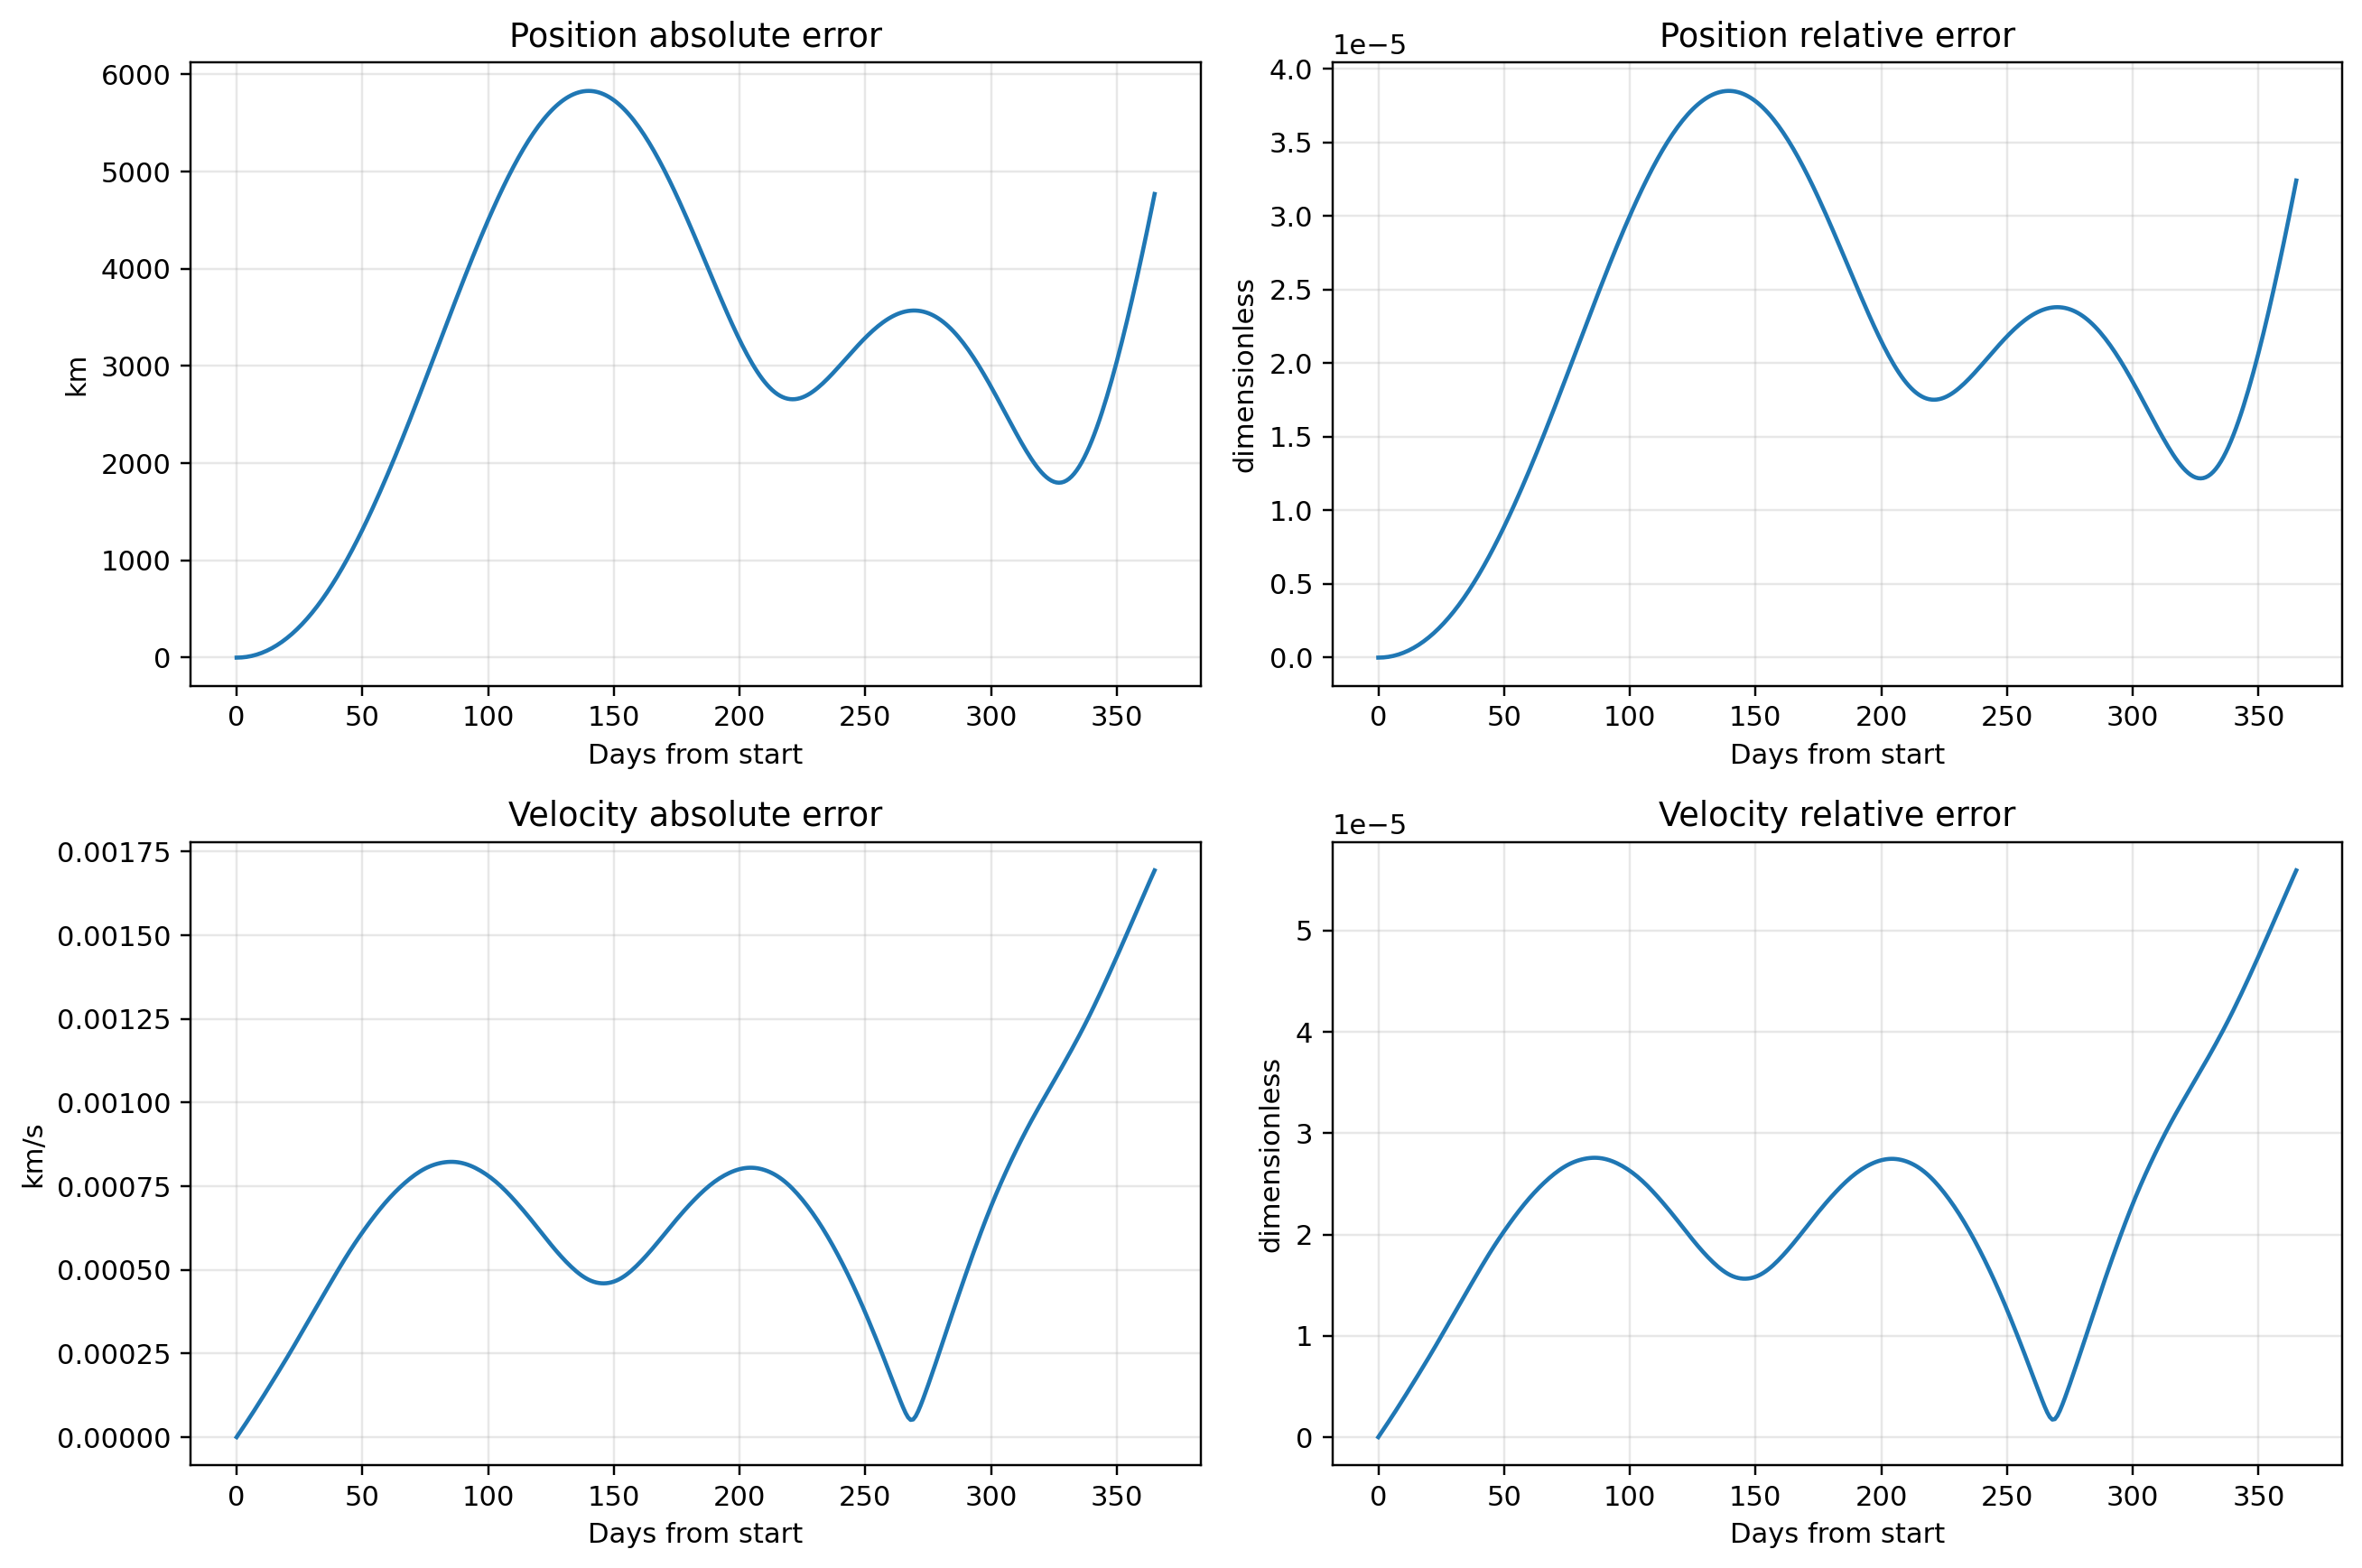
\includegraphics[width=0.95\textwidth]{jpl_compare_output/sun_embary_compare_errors.png}
\caption{Sun--EM Bary 三维二体模型与 JPL Horizons 参考解的误差对比。左上图为位置绝对误差，右上图为位置相对误差，左下图为速度绝对误差，右下图为速度相对误差。可以看到，在一年传播区间内，位置误差整体保持在 \(10^4\ \mathrm{km}\) 以内，速度误差保持在 \(10^{-3}\ \mathrm{km/s}\) 量级；误差曲线呈现明显的周期性起伏，而不是单调爆炸，说明三维二体模型能够较好地捕捉真实 Sun--EM Bary 轨道的主运动特征，但与 JPL 高精度多体星历之间仍存在可观测的系统性偏差。}
\label{fig:sun-embary-jpl-errors}
\end{figure}

\subsection{与 JPL 近似轨道要素的关系}

若不直接使用 Horizons 的向量表，也可先用 JPL 给出的 EM Bary 近似 Kepler 轨道要素作初值近似，然后再与 Horizons 精细数据比较。这样做的逻辑是：
\begin{enumerate}[label=\arabic*.]
  \item 用 JPL 的近似要素给出一个合理的初始椭圆轨道；
  \item 用二体模型数值传播得到轨道；
  \item 用 Horizons 作为高精度参考，检验二体模型在短期和中期内的误差累积。
\end{enumerate}
这比“随意给一个单位圆初值”更接近真实太阳系数据。


\appendix

\section*{附录：关于 JPL 的简要介绍}

JPL 是 \emph{Jet Propulsion Laboratory} 的缩写，中文通常译为“喷气推进实验室”。
它是美国最重要的航天科研机构之一，现由加州理工学院（California Institute of Technology, Caltech）
为美国国家航空航天局（NASA）负责管理和运行。JPL 的起源可以追溯到 20 世纪 30 年代末，
当时加州理工学院教授 Theodore von K\'arm\'an 主持早期火箭推进研究，
Frank Malina 是这一方向最早的学术带头人，而 Jack Parsons 与 Edward Forman 
则是最早参与实验并推动项目落地的核心成员之一。由于这些早期火箭实验常常伴随爆炸与危险操作，
这批研究者在校园中一度被戏称为 \emph{Suicide Squad}（“自杀小队”）\cite{JPLHistory,CaltechLaunchPoints}。

\begin{figure}[htbp]
  \centering
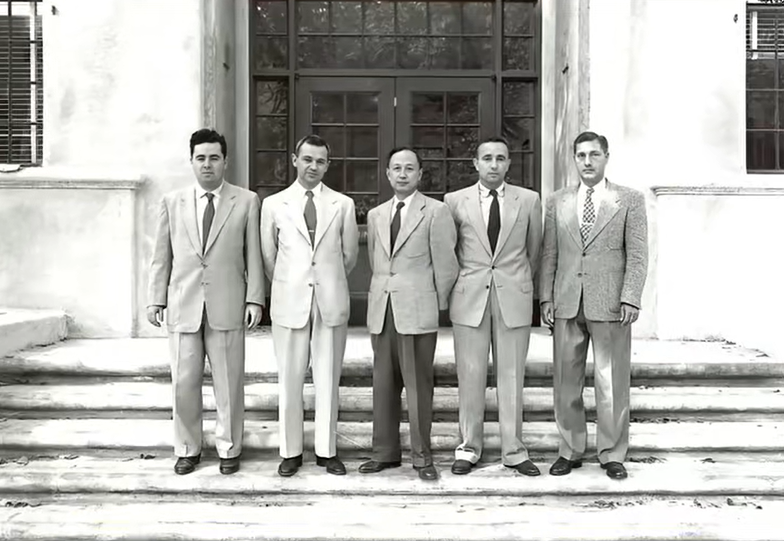
\includegraphics[width=0.75\textwidth]{images/jpl.png}
\caption{照片收藏在 加州理工学院档案馆 (Caltech Archives) 或 JPL 历史档案馆中。
拍摄时间：约 1940年代初（JPL 正式成立前后）。地点：加州理工学院（Caltech）的某处实验楼前。
照片中的人物（从左至右）：阿波罗·史密斯 (Apollo M.O. Smith)：空气动力学专家。
弗兰克·马利纳 (Frank Malina)：JPL 的第一任主管，实验室的学术和组织灵魂。
钱学森 (Tsien Hsue-shen)：理论数学与高速飞行理论专家，JPL 联合创始人，后来的“中国航天之父”。
爱德华·福尔曼 (Edward Forman)：天才机械师，“自杀小队”初创成员之一。
杰克·帕森斯 (Jack Parsons)：化学天才，固体和液体火箭燃料的奠基人\cite{LindaHallTsien2023}。
}  
\end{figure}

值得一提的是，钱学森（Qian Xuesen, Tsien Hsue-shen）也是这一早期团队的重要参与者之一\cite{CaltechLaunchPoints,LindaHallTsien2023,CaltechEASTsien2009}。
他在加州理工学院学习和研究期间加入了这批火箭实验者，并参与了 1943 年提交给美军的一份 proposal；
在该 proposal 中，\emph{Jet Propulsion Laboratory} 这一名称第一次被正式使用。
第二次世界大战期间，这些研究逐步发展为与喷气辅助起飞（jet-assisted takeoff）和火箭推进有关的工程项目，
并最终在 1944 年发展成正式的 JPL。1958 年 NASA 成立后，JPL 转入 NASA 体系，成为其重要的无人深空探测中心\cite{JPLHistory}。

\begin{figure}[htbp]
  \centering
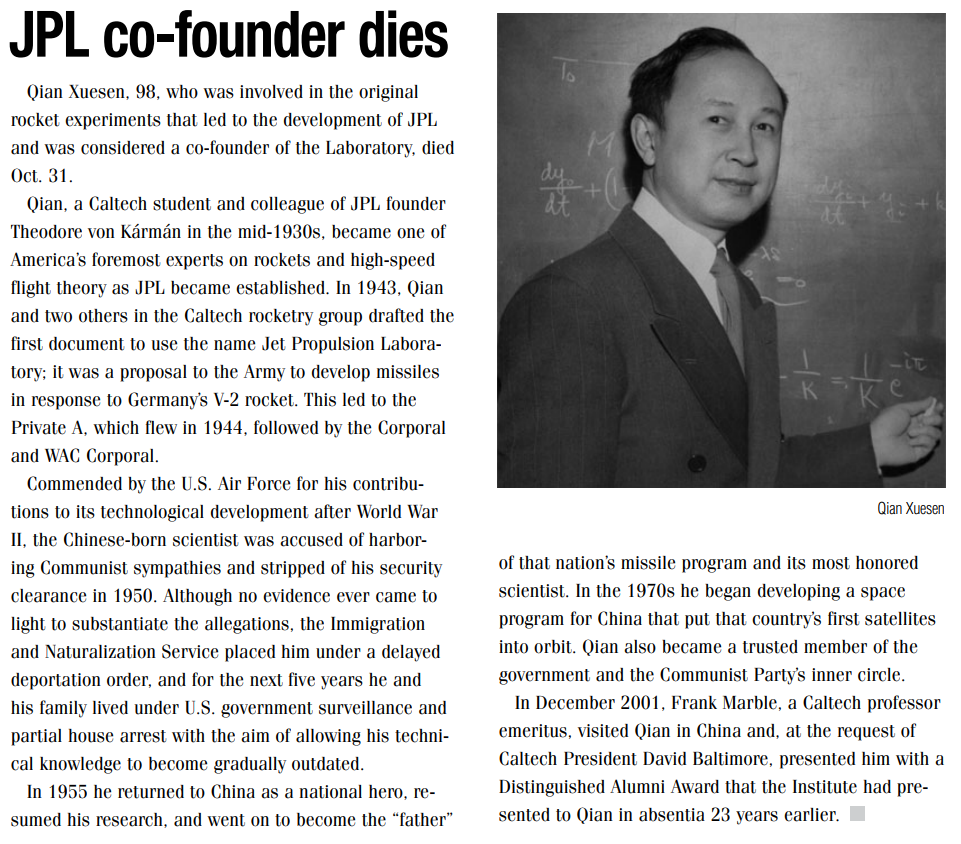
\includegraphics[width=0.75\textwidth]{images/qian.png}
\caption{钱学森去世时加州理工发的悼念公告\cite{CaltechEASTsien2009}}  
\end{figure}


此后，JPL 在美国航天史中发挥了关键作用，参与并主导了多项具有里程碑意义的任务，
例如 \emph{Explorer 1}、\emph{Ranger}、\emph{Surveyor}、\emph{Voyager}、\emph{Galileo}、
\emph{Cassini}、\emph{Mars Pathfinder} 以及后续多代火星探测器等。
今天，JPL 仍然是太阳系探测、深空通信、轨道设计与高精度天体历表计算的重要机构，
其发布的数据与工具在航天工程和天体力学研究中具有广泛影响。

\chapter{JPL Horizons 数据获取示例}

JPL Horizons 是美国喷气推进实验室（Jet Propulsion Laboratory, JPL）
太阳系动力学组提供的一套在线星历与轨道信息服务系统。
它的核心作用是：针对太阳系中的各种天体，按照用户指定的参考中心、参考平面、
时间区间和输出格式，生成高精度的星历、轨道要素以及笛卡尔状态向量。
JPL 官方手册指出，Horizons 面向的对象包括观测者、任务设计人员、研究人员以及公众，
其基本功能是在太阳系范围内，对天体的位置、运动和可观测性随时间的变化进行高精度数值表征。


\section{使用 JPL Horizons API 获取数据的示例}  

以下给出一个便于命令行使用的 Horizons API 示例。为了避免 URL 编码问题，建议使用 \texttt{curl --get} 与 \texttt{--data-urlencode}：

\begin{verbatim}
curl --get "https://ssd.jpl.nasa.gov/api/horizons.api" \
  --data-urlencode "format=text" \
  --data-urlencode "COMMAND='3'" \
  --data-urlencode "CENTER='10'" \
  --data-urlencode "MAKE_EPHEM='YES'" \
  --data-urlencode "EPHEM_TYPE='VECTORS'" \
  --data-urlencode "START_TIME='2026-01-01'" \
  --data-urlencode "STOP_TIME='2026-01-10'" \
  --data-urlencode "STEP_SIZE='1 d'" \
  --data-urlencode "OUT_UNITS='AU-D'" \
  --data-urlencode "REF_PLANE='ECLIPTIC'" \
  --data-urlencode "REF_SYSTEM='J2000'" \
  --data-urlencode "VEC_TABLE='2'" \
  --data-urlencode "CSV_FORMAT='YES'"
\end{verbatim}

其中目标体 \texttt{COMMAND='3'} 表示 Earth--Moon Barycenter，参考中心 \texttt{CENTER='10'} 表示 Sun。
若只想获取某个单独历元的状态，可改用 \texttt{TLIST} 参数并只请求一个时刻。
若希望获取轨道要素而不是状态向量，只需把 \texttt{EPHEM\_TYPE='VECTORS'} 
改为 \texttt{EPHEM\_TYPE='ELEMENTS'}。

\section{天文学数据查询工具 astroquery 简要介绍}

\texttt{astroquery} 是 Python 天文学软件生态中一个常用的数据查询工具包\cite{GinsburgEtAl2019,AstroqueryDocs}，
它属于 Astropy 项目体系中的一个 \emph{coordinated package}。
其主要作用是为研究者提供统一的 Python 接口，以便直接访问各类在线天文数据库和网络服务，
而不必手工编写网页请求或逐条解析返回结果。通过 \texttt{astroquery}，
用户可以较方便地调用诸如 JPL Horizons、SIMBAD、VizieR、MAST 等常见天文数据源，
并将查询结果直接转换为适合后续数值计算和数据分析的结构化对象。

从功能上看，\texttt{astroquery} 的意义在于把原本分散在不同网站和接口中的天文数据服务，
封装为风格较统一的 Python 子模块。例如，在本文所涉及的 Sun--EM Bary 与 JPL Horizons 对比实验中，
就可以通过 \texttt{astroquery.jplhorizons} 直接获取 Earth--Moon Barycenter 相对 Sun 的状态向量，
而不必再手工拼接 URL 或解析复杂的文本输出。这种做法不仅更简洁，也更能减少由于格式解析错误而带来的程序性误差。

在维护机制上，\texttt{astroquery} 并不是某一家公司单独提供的软件，
而是由 Astropy 社区和 Astropy Project 共同维护的开源项目。
作为 Astropy 的 coordinated package，它在整体上接受 Astropy Project 的组织支持，
而具体开发与日常维护则由若干维护者持续推进。正因为如此，\texttt{astroquery} 
已成为天文学 Python 工作流中连接“在线权威数据源”与“本地数值分析程序”的重要桥梁。




\bibliographystyle{plain}
\bibliography{qian}
\end{document}
